\documentclass[11pt]{article}
\usepackage{../EllioStyle}

\title{Homework 1}
\author{Elliott Pryor\\
Worked with: Nathan Stouffer}
\date{24 Jan 2021}

\rhead{Homework 1}
\lhead{Elliott Pryor}

\graphicspath{{./}{images/}}


\makeatletter
\def\mathcolor#1#{\@mathcolor{#1}}
\def\@mathcolor#1#2#3{%
  \protect\leavevmode
  \begingroup
    \color#1{#2}#3%
  \endgroup
}
\makeatother

\newcommand{\pareto}[1]{\rm{Pareto}(#1)}
\newcommand{\conv}[1]{\rm{conv}(#1)}

\begin{document}
\maketitle

\problem{1}
Let $P = \{ p_1, \ldots, p_n \}$ and $P' = \{ p_1', \ldots, p_n' \}$ be the
vertex sets of two upper hulls in the plane.  Each set is presented as a
sequence of points sorted from left to right.  Let $p_i = (x_i, y_i)$ and $p_j'
= (x_j', y_j')$ denote the point coordinates.  We assume that $P$ lies entirely
to the left of $P'$, meaning that there exists a value $z$ such that for all
$i$ and $j$, $x_i < z < x_j'$.

\begin{figure}[h]
    \centering
    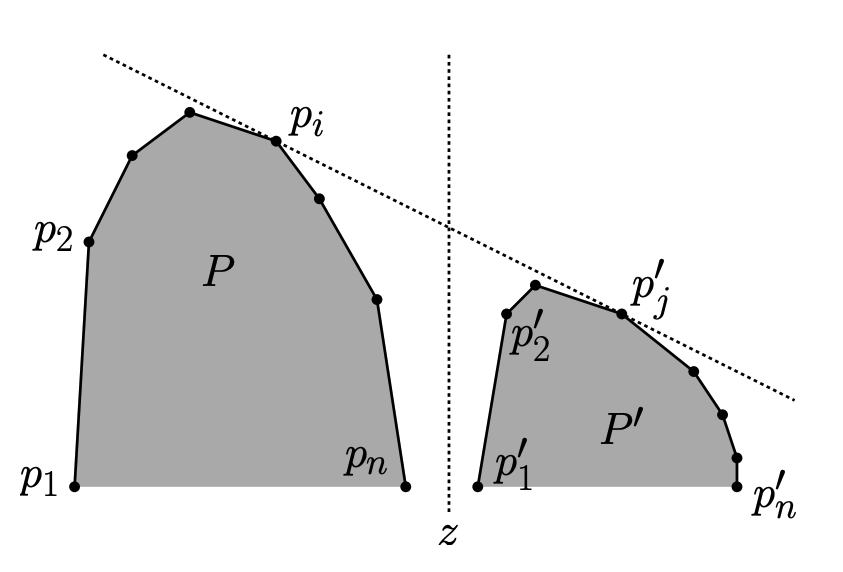
\includegraphics[width=0.5\textwidth]{tangents}
    \caption{Problem 1: Computing the upper tangent of two hulls}
\end{figure}

Present an $O(\log n)$-time algorithm which, given $P$ and $P'$, compute the two
points $p_i \in P$ and $p_j' \in P'$ such that their common support line passes
through these two points.

Briefly justify your algorithm's correctness and drive its running time.  ({\bf
Hint:} The correctness proof involves a case analysis.  Please be careful, a
poorly drawn figure may lead to an incorrect hypothesis.)
\hrule

Some sort of binary search. 

Jointly search P and P'
Pick $a \in P, \sp b \in P'$
Want line with highest z intercept

Idea: O(n) run Grahm's Scan on it. Already sorted so takes O(n) time.

Idea: Start at $a$ compute point $b \in P'$ tangent to $a$ (O (log n)). 
Then reverse, find $a$ tangent to $b$. Then forward, find $b$ tangent to $a$. Then done????

\begin{algorithm}
    \caption{Upper Tangent Function}
    \label{alg:prob1}
    \begin{algorithmic}[1]
    \Function{PeakFinder}{$a, P$}
        \State \textcolor{red}{Binary search to find maximum}
        \State $low \gets 0$
        \State $high \gets |P|$
        \While{!found}
            \State $m \gets \lceil (low + high)/2 \rceil$
            \State $s_1 \gets $ slope of line between $m-1, m$
            \State $s_2 \gets $ slope of line between $m, m+1$
            
            \If{$s_1 > 0$ and $s_2 < 0$}
                \State \textcolor{red}{found peak, slopes make a $\wedge$ at point m}
                \State \textbf{return} $m$
            \ElsIf{$s_1 > 0$ and $s_2 > 0$}
                \State \textcolor{red}{Increasing on both sides, need to go more clockwise (right)}
                \State $high \gets m - 1$
            \ElsIf{$s_1 < 0$ and $s_2 < 0$}
                \State \textcolor{red}{Decreasing on both sides, need to go more counter-clockwise (left)}
                \State $low \gets m + 1$
            \EndIf
            
        \EndWhile
    \EndFunction
    \end{algorithmic}

    \begin{algorithmic}[1]
        \Function{UpperTangent}{$P, P'$}
            \State Run Tangent 3 times to find upper tangent.
            \State $a \gets |P|/2$ \quad // Random point in $P$
            \State $b \gets Tangent(a, P')$ \quad // So we can 'see' $p_i$ from $b$
            \State $a \gets Tangent(b, P)$ \quad // Finds $p_i$
            \State $b \gets Tangent(a, P')$ \quad // Finds $p_j$
            \State \textbf{return} $\overrightarrow{a,b}$
        \EndFunction
        \end{algorithmic}

\end{algorithm}












\problem{2}

Consider a set $P = \{p_1, \ldots, p_n \}$ of points in the plane, where $p_i =
(x_i, y_i)$. A \emph{Pareto set} for $P$, denoted $\pareto{P}$, (named after
the Italian engineer and economist Vilfredo Pareto), is a subset of points
$p_i$ such that there is no $p_j \in P (j \neq i)$ such that $x_j \geq x_i$ and
$y_j \geq y_i$.  That is, each point of $\pareto{P}$ has the property that
there is no point of $P$ that is both to the right and above it.

\begin{figure}[h]
    \centering
    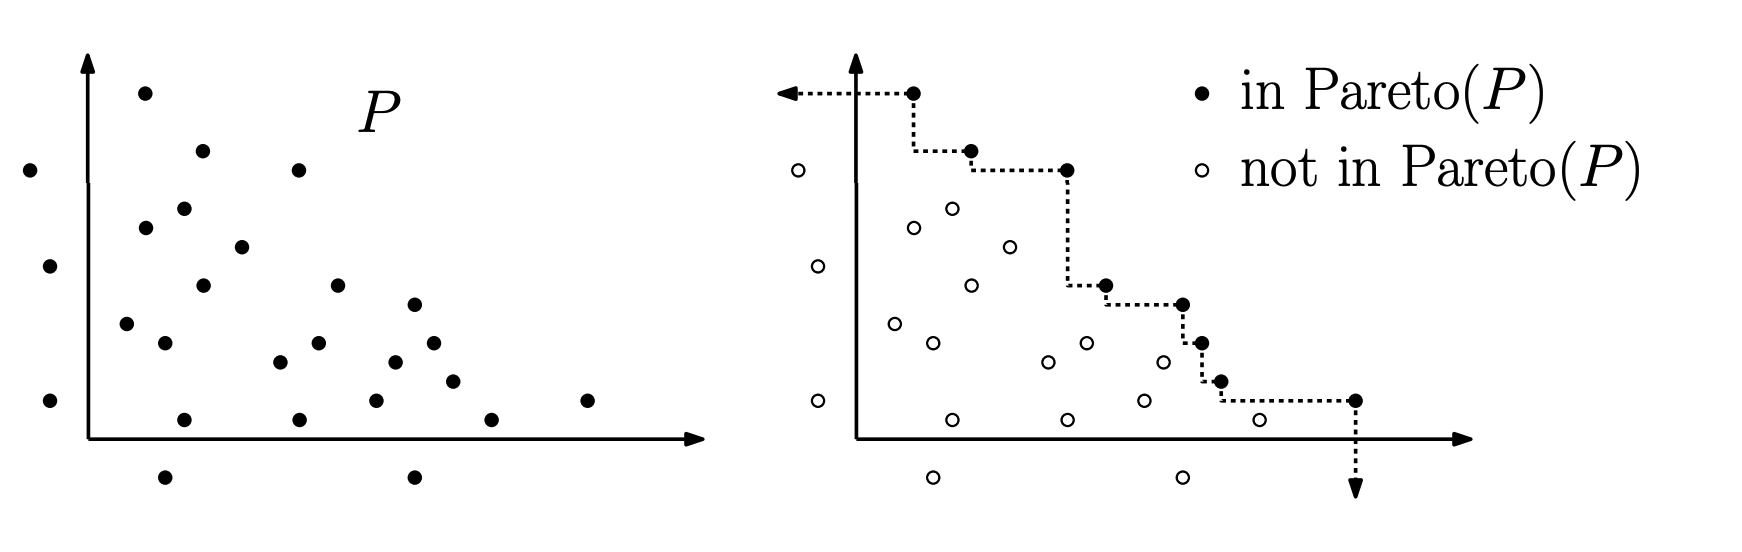
\includegraphics[width=0.75\textwidth]{pareto}
    \caption{Problem 2: Pareto set}
\end{figure}

Pareto sets and convex hulls in the plane are similar in many respects.  In
this problem we will explore some of these connections.

\begin{enumerate}

\item (5 points) A point $p$ lies on the convex hull of a set $P$ if and only if there is
a line passing though $p$ such that all the points of $P$ lie on one side of
this line.  Provide an analogous assertion for the points of $\pareto{P}$ in
terms of a different shape.

\item (5 points) Devise an analogue of Graham's convex-hull algorithm for computing
\pareto{P} in $O(n \log n)$ time.  Briefly justify your algorithm's correctness
and derive its running time.  (You do not need to explain the algorithm ``from
scratch'', that is, you can explain with modifications would be made to Grahm's
algorithm.)

\item (5 points) Devise an analogue of the Jarvis march algorithm for computing
$\pareto{P}$ in $O(h \cdot n)$ time, where $h$ is the cardinality of
$\pareto{P}$.  (As with the previous part, you can just explain the differences
with Jarvis's algorithm.)

\item (5 points) Devise an algorithm for computing $\pareto{P}$ in $O(n
\log h)$ time, where $h$ is the cardinality of $\pareto{P}$.

\end{enumerate}

\hrule

\begin{enumerate}[1. ]
    \item The points on the $Pareto(P)$ fall on a series of horizontal and vertical line segments.
    It follows a line in 'Manhattan' distance. In order to make the analogous assertion,
    we define corner $C(p)$ $p \in P$ as the region $(x,y) \in \reals ^2 \sp x \leq p_x, \sp y \leq p_y$.
    

    Then a point $p$ is on the Pareto of a set $P$ if and only if
    there is no other corner $C(p'), \sp p \neq p'$, containing $p$

    \item 
    This is almost identical to Grahm's Scan. We replace the Orient() function with a different comparison.
    We simply compare the $y$ values of adjacent points. Since the points are in sorted, $x$, order
    if a a point $p_i$ has a larger y-coordinate than $p_{i-1}$ the $p_{i-1}$ would be in $C(p_i)$ so is not on the Pareto.
    Since this comparison only needs the first point in the stack, we also adjust initialization of $S$
    to only push $p_1$ onto the stack, and to not terminate the while loop unless there are $0$ points in the stack.
    
    This has the same running time as Grahm's Scam. Since after sorting, the algorithm takes a linear pass through
    all of the points. It also only pops a point at most once from the stack. The only difference with this algorithm
    from Grahm's Scan is the Orient. Since comparing y-coordinates is also a constant time lookup, our running time is $O(n log(n))$
    due to the sorting in line 2.
    \begin{algorithm}
        \caption{Pareto Scan}
        \label{alg:pareto}
        \begin{algorithmic}[1]
        \Function{ParetoScan}{$P$}
            \State sort $P$ by increasing $x$ value
            \State push $p_1$ onto stack $S$
            \For{$i \gets 2,..., n$}
                \While{$|S| \geq 1$ and $p_{i,y} \geq S[top]_y$}
                    \State pop $S$
                \EndWhile
                \State push $p_i$ onto $S$
            \EndFor
        \EndFunction
        \end{algorithmic}
    \end{algorithm}

    \textbf{Correctness:} We show that algorithm \ref{alg:pareto} is correct by induction. 
    A pareto front is at least one point, so initialization is trivially true.

    We assume that the points on the stack are the pareto front for the first $i-1$ points in $P$.

    Then, we consider point $p_i$. We have two cases. If $p_{i,y} < S[top]_y$ then, since points are in sorted $x$ order,
    $p$ is not in the corner of any of the points of $S$, and none of the points of $S$ are in the corner of $p$. Thus, $S \cup p$
    is the pareto front for the first $i$ points.

    Second, if $p_{i,y} \geq S[top]_y$, then $S[top]$ is in the corner of $p$ (since in sorted $x$ order). Then,
    $S$ gets popped (all popped points meet the above condition) until $|S| < 1$ or $S[top]_y > p_{i,y}$. Thus only points in the corner of $p_i$
    were popped, so are not on the pareto front. Now our stack either has size $1$ from pushing $p$ and is trivially a pareto front. 
    Or it is a valid pareto front for the first $i$ points since it now meets the first condition.

    Thus at the end of the loop, $S$ is a valid pareto front for the first $n$ datapoints, and is thus a valid pareto.

    \item Our modified Jarvis march algorithm would search for the point with the greatest $y$ value.
    Then it would loop and search for the point with the next greatest y-coordinate to the right of the previous point ($p_{i,x} > p_{i-1,x}$).
    This loop is repeated $h - 1$ times (the first point was found in initialization step of finding point with largest y-coordinate).

    \begin{algorithm}
        \caption{Jarvis Stairs}
        \label{alg:jarvis_stairs}
        \begin{algorithmic}[1]
        \Function{JarvisStairs}{$P$}
            \State find point $p_1$ with largest y-coordinate
            \State $S \gets p_1$
            \For{$i \gets 2,..., h$}
                \State find point $p_i$ with largest y-coordinate such that $p_{i,x} > p_{i-1,x}$
            \EndFor
            \State \textbf{return} S
        \EndFunction
        \end{algorithmic}
    \end{algorithm}

    \textbf{Correctness:} The point with the maximum $y$ value must be a part of the pareto. So at initialization we find the point.
    We then search for the next greatest point to the right of this. This point is also part of the pareto. 
    We repeat this $h$ times to find the $h$ points with greatest $y$ value to the right of the previous point. 

    \item We start by dividing $P$ into $n/h$ sets of size $h$. 
    We run Pareto Scan (Algorithm \ref{alg:pareto}) on each of the $n/h$ sets.
    The runtime of this step is $O(h \log(h))$ repeated $n/h$ times: $O(n \log (h))$.

    We can then merge these in $O(n)$ time. We examine this in a 2D matrix. Each row is an individual pareto, and they are all at most $h$ long.
    The algorithm explores this entire matrix, which is $n/h \times h$. So covering this entire matrix takes $O(n/h \cdot h) = O(n)$ time.

    We can also arrive at this an alternative way. Line 3 takes $O(n \log (h))$. Then the for loop is run $h$ times.
    Line 7 and 8 both take $O(n/h)$ time since they go through each mini-pareto once. Line 9 is constant time.
    So the for loop takes $O(h \cdot n/h) = O(n)$.

    \begin{algorithm}
        \caption{Chan Pareto}
        \label{alg:chan_pareto}
        \begin{algorithmic}[1]
        \Function{ChanPareto}{$P$}
            \State divide $P$ into $P_1, P_2, ... P_{n/h}$ where $|P_i| = h$
            \State Solve each $P_i$ using Algorithm \ref{alg:pareto} and store paretos in $S_i$
            \State index $\gets$ list of $n/h$ ones. 
            \State initilize stack $S$
            \For{$1, ... h$}
                \State find point $p$ with largest $y$ coordinate along the indicies ($S_i[index[i]]$)
                \State Go through paretos along indicies and increment index if point $S_i[index[i]]$ is in corner of $p$
                \State push $p$ onto $S$
            \EndFor
            \State \textbf{return} S
        \EndFunction
        \end{algorithmic}
    \end{algorithm}

    \textbf{Correctness:} We know that each mini-pareto is correct since Algorithm \ref{alg:pareto} is correct.
    So we need to show that the merge operation is correct. We know that points on the pareto are part of the mini paretos. 
    By induction, we start with an empty set which is vacuously true. Then we assume that we have the first $i-1$ points of the pareto. 
    And that $index[i]$ points to the largest uncovered point in pareto $S_i$. 

    We show that this holds after the $i^{th}$ iteration. To do this, we show that the point $p$ with the largest $y$ coordinate is part of the pareto.
    By our choice of $p$, it is certainly not covered by any of the points on $S_i[index[i]]$. Thus, we show that it is also not covered by any previous point, or future point.
    By the inductive assumption, $p$ is not covered by any of the points in $S$. 
    Then, suppose that $p$ is covered by a future point $p_j$, that future point would also cover $S_j[index[j]]$. Then $S_j$
    would not be a valid pareto, a contradiction. So $p$ belongs on the pareto. 


\end{enumerate}





\problem{3}

Assume you have an orientation test available which can determine in constant
time whether three points make a left turn (i.e., the third point lies on the
left of the oriented line described by the first two points) or a right turn.
Now, let a point $q$ and a convex polygon $P = \{ p_1, \ldots , p_n \}$ in the
plane be given, where the points of $P$ are stored in an array in
counter-clockwise order around $P$ and $q$ is outside of $P$. Give pseudo-code
to determine the tangents from $q$ to $P$ in $O(\log n)$ time.

\hrule

We say $Orient(a,b,c) > 0$ if it is oriented counter clockwise (makes left turn), and $Orient(a,b,c) < 0$ if it is oriented clockwise (right turn)

\begin{algorithm}
    \caption{Tangent Function}
    \label{alg:prob1}
    \begin{algorithmic}[1]
    \Function{Tangent}{$a, P$}
        \State Binary search to find point of tangency
        \State $low \gets 1$
        \State $high \gets |P|$
        \State $p_1$, $p_2$
        \While{!found}
            \State $c \gets \lceil (low + high)/2 \rceil$
            \State $b \gets c-1, \sp d \gets c + 1$ \quad \textcolor{red}{b is point counter-clockwise from a, d is point clockwise from a}
            \If{$Orient(a, c, b) = Orient(a, c, d)$}
                \State found tangen$t$
                \State $p_1 \gets m$
                \State \textbf{break while}
            \ElsIf{orientations at $c$, $low$, $high$, all match}
                \State \textcolor{red}{this catches if both tangents are on one side of $c$}, 
                \State \textcolor{red}{so we need to go around so we don't get stuck on $low$, or $high$}
                \State move in opposite direction of $Orient(a, c, low)$ and adjust $low, high$ accordingly 
                \State \textcolor{red}{(same as lower rules)}
            \ElsIf{$Orient(a,c,b) > 0$ and $Orient(a,c,d) < 0$}
                \State \textcolor{red}{Need to move search point left (counter-clockwise)}
                \State $high \gets b$
            \ElsIf{$Orient(a,c,b) < 0$ and $Orient(a,c,d > 0)$}
                \State \textcolor{red}{need to move search point right (clockwise)}
                \State $low \gets d$
            \EndIf
        \EndWhile

        \State Repeat same while loop but flipping inequality signs to find other tangency point.
        \State \textbf{return} $p_1, p_2$
    \EndFunction
    \end{algorithmic}
\end{algorithm}


This follows a binary search. Every operation within the while loop takes $O(1)$ time. Then, the same as regular binary search,
the algorithm jumps $(high-low)/2$ every iteration, so it covers the entire list in $O(\log (n))$ time. 

\textbf{Correctness:} 
We use Figure \ref{fig:orientation} to justify the rules in the else if statements lines 18-23.
This shows the orientation values when we need to move clockwise and counter-clockwise.
\begin{figure}[h]
    \centering
    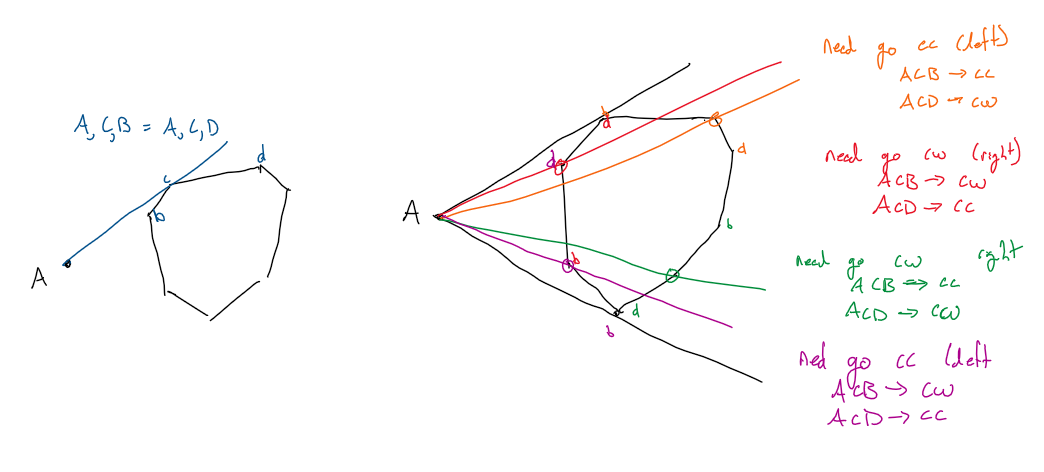
\includegraphics[width=0.9\textwidth]{prob_3_correctness.png}
    \caption{Orientation Rules Justification and example}
    \label{fig:orientation}
\end{figure}

The else if statement line 12-17 is used to catch the edge case where both tangents are on one side of our center line.
This means that if we listen to the normal rules in the other else if statements, we may get caught and unable to pass our high or low marker. 
This case occurs when all 3 points are on one 'face', so we know that we will get trapped moving towards them.
So we move in the opposite direction. This will eventually put c in between the two tangents and the algorithm will work normally.


\problem{4}

Given a set $S$ of $n$ points in the plane, consider the subsets

\begin{eqnarray*}
	S_1 &=& S, \\
	S_2 &=& S_1 \setminus \{ \text{set of vertices of } \conv{S_1} \} \\
		&\ldots& \\
	S_i &=& S_{i-1} \setminus \{ \text{set of vertices of } \conv{S_{i-1}} \}
\end{eqnarray*}
%
until $S_k$ has at most three elements.  Give an $O(n^2)$ time algorithm that
computes all convex hull $\conv{S_1}, \conv{S_2}, \ldots, S_k$.  [Extra credit,
provide an algorithm that is faster than $O(n^2)$].

\begin{figure}[h]
    \centering
    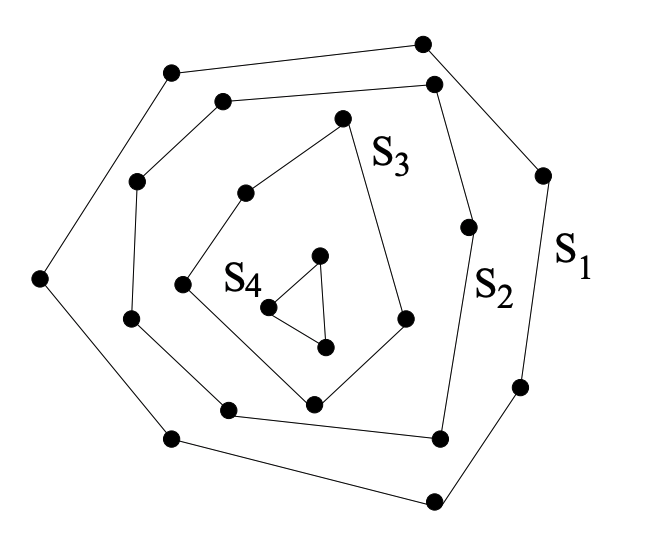
\includegraphics[width=0.25\textwidth]{onions}
    \caption{Problem 4: Onion peeling}
\end{figure}
\hrule

We essentially do Grahm's Scan, but instead of popping and removing them,
we move the popped hull sections down one layer.

So for the runtime, the sort operation takes $O(n \log (n))$. Then at worst case, every single point gets sifted down every shell. 
There are at most $O(n)$ shells. So it takes $O(n^2)$ time.

\begin{algorithm}
    \caption{Onion Problem}
    \label{alg:onion}

    \begin{algorithmic}[1]
        \Function{recurr}{$p', S$}
            \State popped = []
            \While{$|S| \leq 2$ and $Orient(p', S[top], S[top-1]) < 0$}
                \State popped.append($S.pop()$)
            \EndWhile
            \State \textbf{return} popped
        \EndFunction
        \end{algorithmic}

    \begin{algorithmic}[1]
    \Function{Onions}{$P$}
        \State sort $P$ by increasing $x$
        \State push $p_1, p_2$ onto stack $S_0$
        \For{$i \gets 3, ..., n$}
            \State \textcolor{red}{Variable initialization to clean things up}
            \State $S \gets S_0$ 
            \State $add\_to\_next \gets [p_i]$ \quad \textcolor{red}{mark $p_i$ to be added to S}
            \State $popped \gets recurr(p_i,S)$ \quad \textcolor{red}{get points removed from S}
            \While{$popped$ is not empty}
                \State $S.push(add\_to\_next)$ \quad \textcolor{red}{add the points to this shell}
                \State $add\_to\_next \gets popped$
                \State $p' \gets popped[top]$
                \State $S \gets$ next layer down stack
                \State $popped \gets recurr(p', S)$
            \EndWhile
            \State $S.push(add\_to\_next)$ \quad \textcolor{red}{Add to last layer}
        \EndFor
        \State repeat to make the lower hull.
    \EndFunction
    \end{algorithmic}
\end{algorithm}

\textbf{Correctness:} We prove this inductively on each shell. So considering just the outer shell,
we have the exact same as Graham's Scan algorithm, so it is correct. 

Then for each of the lower shells, we take a convex shell segment and add it to the lower shell. 
We show that the shell segment gets added in its entirity.

Suppose not, suppose the entire shell segment $S'$ should not be added. We say the first point in the shell segment is $p$.
And the shell we consider is $S$. Suppose only the first portion of the shell segment can be added without breaking convexity.
Then the remaining portion can be added without breaking convexity since the entire shell segment was convex. 

Then suppose that some point that was popped, should be added partially through the segment. 
This is a contradiction since we are building the upper hull and the points are in sorted order. So any popped point has
$x < p_x$. If we add the popped point back, the sorted $x$ ordering is broken a contradiction.

The inner hulls are also correct since Grahm's Scan is run on each of them.  



\end{document}